\scanpage{51}

\uline{Lemme 1}\quad Soit $k$ un corps algébriquement clos, $K$ une extension de type fini, de degré de transcendance $1$, de $k$. Alors $K$ est \deleted{\unsure{alg.}} quasi-algébriquement clos
\figure{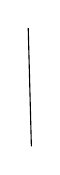
\begin{tikzpicture}[x=1cm,y=1cm]\draw (0,0)--(-.04,1.5);\end{tikzpicture}}

\uline{Corollaire 1}\quad $\widehat H^i(K^{\unsure{a|'}},G_m)=0$ pour tout $i$

En effet, $K$ est une extension galoisienne \unsure{un|d'un} $K'$ est quasi-alg. clos, donc \deleted{$\unsure{\widehat H^i(K,G)}$} la conclusion est bien connue.

\uline{Corollaire 2}\quad $\unsure{\widehat H}^i(K,\Gamma)=0$ \deleted{$i>0$ pour} \inserted{pour tt $i>1$ et} tout groupe abélien fini $\Gamma$ où $G_K$ opère trivialement.
\figure{\begin{tikzpicture}[x=1cm,y=1cm]\draw (0,0)--(-.02,.7);\end{tikzpicture}}

Soit en effet $\widetilde K$ \deleted{la} \inserted{une} clôture galoisienne de $K$,
$[U\subset\widetilde K^*$ \unsure{le} groupe des racines de l'unité dans $\widetilde K$.
Alors $\widetilde K^*/U$ est uniquement divisible sauf pour $p$ (exposant car.) d'où la suite exacte \uline{mod} $p$
\[
\widehat H^i(K,\unsure{U_m|G_m})\xrightarrow{\sim}\widehat H^i(K,G_m)\deleted{\text{\unsure{mod}}\ p}\qquad\uuline{\text{mod }p}
\]
\margin{est-ce $\unsure{\simeq|=}$ un vrai isomorphisme?}
\figure{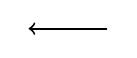
\begin{tikzpicture}[x=1cm,y=1cm]\draw[->,line width=.7pt] (1,0)--(0,0);\end{tikzpicture}}
Or le \deleted{premier} deuxième mb. est nul, donc le premier l'est, donc comme le premier \deleted{\unsure{n'a que}} a $p$-composante nulle, il est nul.$]$
On \deleted{\unsure{en déduit}} \inserted{\deleted{peut} voit} plus précisément que si $n$ est premier à la caractéristique, alors
\diagram{\begin{tikzcd}\widetilde K\arrow[r,"x\to x^n"]&\widetilde K^{\unsure{n}}\end{tikzcd}}
est un épimorphisme de \deleted{groupe de} noyau $\simeq\mathbb Z/n$, donc la suite exacte de cohomologie donne le résultat $H^i(K,\unsure{\mathbb Z_n|\mathbb Z/n})=0$.

Reste à prouver $H^i(K,\mathbb Z/p)=0$ si $i>1$. Pour ceci
\deleted{\uline{Lemme 2} Soit}
on considère la suite exacte
\diagram{\begin{tikzcd}0\arrow[r]&\unsure{\mathbb Z}/p\arrow[r,no head]&\widetilde K\arrow[r,"\wp"]&\unsure{\widetilde K'|\widetilde K}\arrow[r]&0\end{tikzcd}}.

\mspage{50}

